\newpage
\section{Recommendations on practical settings}
\label{section:PracticalSettings}


\subsection{Webservers}

\subsubsection{Apache}

\begin{description}
\item[Tested with Version:]

\item[Settings:] \mbox{}

%-All +TLSv1.1 +TLSv1.2
\begin{lstlisting}[breaklines]
  SSLProtocol All -SSLv2 -SSLv3 
  SSLHonorCipherOrder On
  SSLCompression off
  # Add six earth month HSTS header for all users...
  Header add Strict-Transport-Security "max-age=15768000"
  # If you want to protect all subdomains, use the following header
  # ALL subdomains HAVE TO support https if you use this!
  # Strict-Transport-Security: max-age=15768000 ; includeSubDomains

  SSLCipherSuite 'EECDH+aRSA+AESGCM:EECDH+aRSA+SHA384:EECDH+aRSA+SHA256:EDH+CAMELLIA256:EECDH:EDH+aRSA:+SSLv3:!aNULL:!eNULL:!LOW:!3DES:!MD5:!EXP:!PSK:!SRP:!DSS:!RC4:!SEED:!AES128:!CAMELLIA128:!ECDSA:AES256-SHA'
\end{lstlisting}

Note again, that any cipher suite starting with ECDHE  can be omitted in case of doubt.
%% XXX NOTE TO SELF: remove from future automatically generated lists!

\item[Additional settings:]

You should redirect everything to httpS:// if possible. In Apache you can do this with the following setting inside of a VirtualHost environment:

\begin{lstlisting}[breaklines]
  <VirtualHost *:80>
   #...
   RewriteEngine On
        RewriteRule ^.*$ https://%{SERVER_NAME}%{REQUEST_URI} [L,R=permanent]
   #...
  </VirtualHost>
\end{lstlisting}

\item[Justification for special settings (if needed):]

\item[References:]

\item[How to test:]

See ssllabs in section \ref{section:Tools}

\end{description}
%XXXX   ECDH+AES256:DH+AES256:ECDH+AES128:DH+AES:ECDH+3DES:DH+3DES:RSA+AES:RSA+3DES:!ADH:!AECDH:!MD5:!DSS


\subsubsection{lighttpd}



\begin{description}
\item[Tested with Version:]

\todo{version?}

\item[Settings:] \mbox{}


%% Complete ssl.cipher-list with same algo than Apache
\todo{FIXME: this string seems to be wrongly formatted??}

\begin{lstlisting}[breaklines]
  $SERVER["socket"] == "0.0.0.0:443" {
    ssl.engine  = "enable"
    ssl.use-sslv2 = "disable"
    ssl.use-sslv3 = "disable"
    #ssl.use-compression obsolete >= 1.4.3.1
    ssl.pemfile = "/etc/lighttpd/server.pem"
    ssl.cipher-list = 'EECDH+aRSA+AESGCM:EECDH+aRSA+SHA384:EECDH+aRSA+SHA256:EDH+CAMELLIA256:EECDH:EDH+aRSA:+SSLv3:!aNULL:!eNULL:!LOW:!3DES:!MD5:!EXP:!PSK:!SRP:!DSS:!RC4:!SEED:!AES128:!CAMELLIA128:!ECDSA:AES256-SHA'
    ssl.honor-cipher-order = "enable"
    setenv.add-response-header  = ( "Strict-Transport-Security" => "max-age=31536000")
  }
\end{lstlisting}


\item[Additional settings:]

As for any other webserver, you should redirect automatically http traffic toward httpS://

\begin{lstlisting}[breaklines]
  $HTTP["scheme"] == "http" {
    # capture vhost name with regex conditiona -> %0 in redirect pattern
    # must be the most inner block to the redirect rule
    $HTTP["host"] =~ ".*" {
        url.redirect = (".*" => "https://%0$0")
    }
  }
\end{lstlisting}


\item[References:] 
\todo{add references}.
lighttpd httpS:// redirection: \url{http://redmine.lighttpd.net/projects/1/wiki/HowToRedirectHttpToHttps}

% add any further references or best practice documents here

\item[How to test:] See ssllabs in section \ref{section:Tools}

% describe here or point the admin to tools (can be a simple footnote or \ref{} to  the tools section) which help the admin to test his settings.
\end{description}


\subsubsection{nginx}

\begin{description}
\item[Tested with Version:]

\todo{version?}

\item[Settings:] \mbox{}

\begin{lstlisting}[breaklines]
  ssl_prefer_server_ciphers on;
  ssl_protocols -SSLv2 -SSLv3; 
  ssl_ciphers 'EECDH+aRSA+AESGCM:EECDH+aRSA+SHA384:EECDH+aRSA+SHA256:EDH+CAMELLIA256:EECDH:EDH+aRSA:+SSLv3:!aNULL:!eNULL:!LOW:!3DES:!MD5:!EXP:!PSK:!SRP:!DSS:!RC4:!SEED:!AES128:!CAMELLIA128:!ECDSA:AES256-SHA';
  add_header Strict-Transport-Security max-age=2592000;
  add_header X-Frame-Options DENY;
\end{lstlisting}

%% XXX FIXME: do we need to specify dhparams? Parameter: ssl_dhparam = file. See: http://wiki.nginx.org/HttpSslModule#ssl_protocols

\item[Additional settings:]

If you decide to trust NIST's ECC curve recommendation, you can add the following line to nginx's configuration file to select special curves:

\begin{lstlisting}[breaklines]
  ssl_ecdh_curve          sect571k1;
\end{lstlisting}

You should redirect everything to httpS:// if possible. In Nginx you can do this with the following setting:

\begin{lstlisting}[breaklines]
  rewrite     ^(.*)   https://$host$1 permanent;
\end{lstlisting}


\item[References:] \todo{add references}

\item[How to test:] See ssllabs in section \ref{section:Tools}

\end{description}





\subsubsection{MS IIS}
\label{sec:ms-iis}


\todo{Daniel: add screenshots and registry keys}

\begin{description}

\item[Tested with Version:] \todo{Daniel: add tested version}

\item[Settings:] \mbox{}


When trying to avoid RC4 and CBC (BEAST-Attack) and requiring perfect
forward secrecy, Microsoft Internet Information Server (IIS) supports
ECDSA, but does not support RSA for key exchange (consider ECC suite
B doubts\footnote{\url{http://safecurves.cr.yp.to/rigid.html}}).

Since \verb|ECDHE_RSA_*| is not supported, a SSL certificate based on
elliptic curves needs to be used.

The configuration of cipher suites MS IIS will use can be configured in one
of the following ways:
\begin{enumerate}
\item Group Policy \footnote{\url{http://msdn.microsoft.com/en-us/library/windows/desktop/bb870930(v=vs.85).aspx}}
\item Registry
\item IIS Crypto~\footnote{\url{https://www.nartac.com/Products/IISCrypto/}}
\end{enumerate}


Table~\ref{tab:MS_IIS_Client_Support} shows the process of turning on
one algorithm after another and the effect on the supported Clients
tested using https://www.ssllabs.com.

\verb|SSL 3.0|, \verb|SSL 2.0| and \verb|MD5| are turned off.
\verb|TLS 1.0| and \verb|TLS 2.0| are turned on.

\begin{table}[h]
  \centering
  \small
  \begin{tabular}{ll}
    \toprule
    Cipher Suite & Client \\
    \midrule
    \verb|TLS_ECDHE_ECDSA_WITH_AES_128_GCM_SHA256| & only IE 10,11, OpenSSL 1.0.1e \\
    \verb|TLS_ECDHE_ECDSA_WITH_AES_128_CBC_SHA256| & Chrome 30, Opera 17, Safari 6+ \\
    \verb|TLS_ECDHE_ECDSA_WITH_AES_128_CBC_SHA| & FF 10-24, IE 8+, Safari 5, Java 7\\
    \bottomrule 
 \end{tabular}
  \caption{Client support}
  \label{tab:MS_IIS_Client_Support}
\end{table}

Table~\ref{tab:MS_IIS_Client_Support} shows the algoriths from
strongest to weakest and why they need to be added in this order. For
example insisting on SHA-2 algorithms (only first two lines) would
eliminate all versions of Firefox, so the last line is needed to
support this browser, but should be placed at the bottom, so capable
browsers will choose the stronger SHA-2 algorithms.

\verb|TLS_RSA_WITH_RC4_128_SHA| or equivalent should also be added if
MS Terminal Server Connection is used (make sure to use this only in a
trusted environment). This suite will not be used for SSL, since we do
not use a RSA Key.


% \verb|TLS_ECDHE_ECDSA_WITH_AES_128_GCM_SHA256| ... only supported by: IE 10,11, OpenSSL 1.0.1e
% \verb|TLS_ECDHE_ECDSA_WITH_AES_128_CBC_SHA256| ... Chrome 30, Opera 17, Safari 6+
% \verb|TLS_ECDHE_ECDSA_WITH_AES_128_CBC_SHA| ... Firefox 10-24, IE 8+, Safari 5, Java 7


Not supported Clients:
\begin{enumerate}
\item Java 6
\item WinXP
\item Bing
\end{enumerate}

\item[Additional settings:]

%Here you can add additional settings

\item[Justification for special settings (if needed):]

% in case you have the need for further justifications why you chose this and that setting or if the settings do not fit into the standard Variant A or Variant B schema, please document this here

\item[References:]

\todo{add references}

% add any further references or best practice documents here

\item[How to test:] See ssllabs in section \ref{section:Tools}


\end{description}



\subsection{Mail Servers}

This section documents the most common mail (SMTP) and IMAPs/POPs servers. Another option to secure IMAPs/POPs servers is to place them behind an stunnel server. 

\subsubsection{Dovecot}


Dovecot 2.2:

% Example: http://dovecot.org/list/dovecot/2013-October/092999.html

\begin{lstlisting}[breaklines]
  ssl_cipher_list = 'EECDH+aRSA+AESGCM:EECDH+aRSA+SHA384:EECDH+aRSA+SHA256:EDH+CAMELLIA256:EECDH:EDH+aRSA:+SSLv3:!aNULL:!eNULL:!LOW:!3DES:!MD5:!EXP:!PSK:!SRP:!DSS:!RC4:!SEED:!AES128:!CAMELLIA128:!ECDSA:AES256-SHA'
  ssl_prefer_server_ciphers = yes
\end{lstlisting}

Dovecot 2.1: Almost as good as dovecot 2.2. Does not support ssl\_prefer\_server\_ciphers

\paragraph*{Limitations}\mbox{}\\

Dovecot currently does not support disabling TLS compression. Furthermore, DH parameters
greater than 1024bit aren't possible. The most recent version 2.2.7 of Dovecot implements
configurable DH parameter length
\footnote{\url{http://hg.dovecot.org/dovecot-2.2/rev/43ab5abeb8f0}}.

\subsubsection{cyrus-imapd (based on 2.4.17)}

\paragraph*{imapd.conf}\mbox{}\\

To activate SSL/TLS configure your certificate with
\begin{lstlisting}[breaklines]
  tls_cert_file: .../cert.pem
  tls_key_file: .../cert.key
\end{lstlisting}

Do not forget to add necessary intermediate certificates to the .pem file.\\

Limiting the ciphers provided may force (especially older) clients to connect without encryption at all! Sticking to the defaults is recommended.\\

If you still want to force strong encryption use
\begin{lstlisting}[breaklines]
  tls_cipher_list: <...recommended ciphersuite...>
\end{lstlisting}

cyrus-imapd loads hardcoded 1024 bit DH parameters using get\_rfc2409\_prime\_1024() by default. If you want to load your own DH parameters add them PEM encoded to the certificate file given in tls\_cert\_file. Do not forget to re-add them after updating your certificate.\\

To prevent unencrypted connections on the STARTTLS ports you can set
\begin{lstlisting}[breaklines]
  allowplaintext: 0
\end{lstlisting}
This way MUAs can only authenticate after STARTTLS if you only provide plaintext and SASL PLAIN login methods. Therefore providing CRAM-MD5 or DIGEST-MD5 methods is not recommended.\\

\paragraph*{cyrus.conf}\mbox{}\\

To support POP3/IMAP on ports 110/143 with STARTTLS add
\begin{lstlisting}[breaklines]
  imap         cmd="imapd" listen="imap" prefork=3
  pop3         cmd="pop3d" listen="pop3" prefork=1
\end{lstlisting}
to the SERVICES section.\\

To support POP3S/IMAPS on ports 995/993 add
\begin{lstlisting}[breaklines]
  imaps        cmd="imapd -s" listen="imaps" prefork=3
  pop3s        cmd="pop3d -s" listen="pop3s" prefork=1
\end{lstlisting}


\paragraph*{Limitations}\mbox{}\\

cyrus-imapd currently (2.4.17, trunk) does not support elliptic curves. ECDHE will not work even if defined in your cipher list.\\

Currently there is no way to prefer server ciphers or to disable compression.\\

There is a working patch for all three features:
\url{https://bugzilla.cyrusimap.org/show_bug.cgi?id=3823}\\





% XXX config von Adi?
% sslVersion = TLSv1
% ciphers = EDH+CAMELLIA256:EDH+aRSA:+SSLv3:!aNULL:!eNULL:!LOW:!3DES:!MD5:!EXP:!PSK:!SRP:!DSS:!RC4:!SEED:-AES128:!CAMELLIA128:!ECDSA:AES256-SHA:EDH+AES128;
% options = CIPHER_SERVER_PREFERENCE
% TIMEOUTclose = 1

\subsubsection{SMTP in general}

SMTP usually uses opportunistic TLS. This means that an MTA will accept TLS connections when asked for it during handshake but will not require it. One should always support incoming opportunistic TLS and always try TLS handshake outgoing.\\

Furthermore a mailserver can operate in three modes:
\begin{itemize}
\item As MSA (Mail Submission Agent) your mailserver receives mail from your clients MUAs (Mail User Agent).
\item As receiving MTA (Mail Transmission Agent, MX)
\item As sending MTA (SMTP client)
\end{itemize}
\mbox{}\\
We recommend the following basic setup for all modes:
\begin{itemize}
\item correctly setup MX, A and PTR RRs without using CNAMEs at all.
\item enable encryption (opportunistic TLS)
\item do not use self signed certificates
\end{itemize}

For SMTP client mode we additionally recommend:
\begin{itemize}
\item the hostname used as HELO must match the PTR RR
\item setup a client certificate (most server certificates are client certificates as well)
\item either the common name or at least an alternate subject name of your certificate must match the PTR RR
\item do not modify the cipher suite for client mode
\end{itemize}

For MSA operation we recommend:
\begin{itemize}
\item listen on submission port 587
\item enforce SMTP AUTH even for local networks
\item do not allow SMTP AUTH on unencrypted connections
\item optionally use the recommended cipher suites if (and only if) all your connecting MUAs support them
\end{itemize}



% Note that (with the exception of MSA mode), it might be better to allow any cipher suite -- since any encryption is better than no encryption when it comes to opportunistic TLS.

We strongly recommend to allow all cipher suites for anything but MSA
mode, because the alternative is plain text transmission.

\subsubsection{Postfix}

\begin{description}
\item[Tested with Version:] \mbox{}

\begin{itemize}
\item Postfix 2.9.6 (Debian Wheezy)
\end{itemize}

\item[Settings:] \mbox{}

First, you need to generate Diffie Hellman parameters (please first take a look at the section \ref{section:PRNG}):

\todo{FIXME: this is a really weak setting! See also: http://postfix.1071664.n5.nabble.com/postfix-hardening-what-can-we-do-td61874.html}
\begin{lstlisting}[breaklines]
  % openssl gendh -out /etc/postfix/dh_param_512.pem -2 512
  % openssl gendh -out /etc/postfix/dh_param_1024.pem -2 1024
\end{lstlisting}

Next, we specify these DH parameters in \verb|main.cf|:

\begin{lstlisting}[breaklines]
  smtpd_tls_dh512_param_file = /etc/postfix/dh_param_512.pem
  smtpd_tls_dh1024_param_file = /etc/postfix/dh_param_1024.pem
\end{lstlisting}

\paragraph*{MX and SMTP client configuration}\mbox{}\\

As discussed above, because of opportunistic encryption we do not
restrict the list of ciphers. There's still some steps needed to
enable TLS, all in \verb|main.cf|:

\begin{lstlisting}[breaklines]
  smtpd_tls_cert_file = /etc/postfix/server.pem
  smtpd_tls_key_file = /etc/postfix/server.key
  # use 0 for Postfix >= 2.9, and 1 for earlier versions
  smtpd_tls_loglevel = 0
  # enable opportunistic TLS support in the SMTP server and client
  smtpd_tls_security_level = may
  smtp_tls_security_level = may
  # if you have authentication enabled, only offer it after STARTTLS
  smtpd_tls_auth_only = yes
  tls_ssl_options=NO_COMPRESSION
  tls_random_source = dev:/dev/urandom		
\end{lstlisting}

\paragraph*{MSA}\mbox{}\\

For the MSA \verb|smtpd| process, we first define the ciphers that are
acceptable for the ``mandatory'' security level, again in
\verb|main.cf|:

\begin{lstlisting}[breaklines]
  smtpd_tls_mandatory_protocols = !SSLv2, !SSLv3
  smtpd_tls_mandatory_ciphers=high
  tls_high_cipherlist=EECDH+aRSA+AESGCM:EECDH+aRSA+SHA384:EECDH+aRSA+SHA256:EDH+CAMELLIA256:EECDH:EDH+aRSA:+SSLv3:!aNULL:!eNULL:!LOW:!3DES:!MD5:!EXP:!PSK:!SRP:!DSS:!RC4:!SEED:!AES128:!CAMELLIA128:!ECDSA:AES256-SHA
\end{lstlisting}

Then, we configure the MSA smtpd in \verb|master.cf| with two
additional options that are only used for this instance of smtpd:

\begin{lstlisting}[breaklines]
587       inet  n       -       -       -       -       smtpd 
        -o smtpd_tls_security_level=encrypt -o tls_preempt_cipherlist = yes
\end{lstlisting}

For those users who want to use ECC key exchange, it is possible to specify this via:
\begin{lstlisting}[breaklines]
  smtpd_tls_eecdh_grade = ultra
\end{lstlisting}

\item[Limitations:] \mbox{}

tls\_ssl\_options is supported from Postfix 2.11 onwards. You can
leave the statement in the configuration for older versions, it will
be ignored.

tls\_preempt\_cipherlist is supported from Postfix 2.8 onwards. Again,
you can leave the statement in for older versions.

\item[References:]

Refer to \url{http://www.postfix.org/TLS_README.html} for an in-depth
discussion.

% \item[Additional settings:]
% no additional settings

% \item[Justification for special settings (if needed):]
% no special settings

\item[How to test:]

You can check the effect of the settings with the following command:
\begin{lstlisting}[breaklines]
$ zegrep "TLS connection established from.*with cipher" | /var/log/mail.log | awk '{printf("%s %s %s %s\n", $12, $13, $14, $15)}' | sort | uniq -c | sort -n
      1 SSLv3 with cipher DHE-RSA-AES256-SHA
     23 TLSv1.2 with cipher DHE-RSA-AES256-GCM-SHA384
     60 TLSv1 with cipher ECDHE-RSA-AES256-SHA
    270 TLSv1.2 with cipher ECDHE-RSA-AES256-GCM-SHA384
    335 TLSv1 with cipher DHE-RSA-AES256-SHA
\end{lstlisting}

\end{description}

\subsubsection{Exim (based on 4.82)}

It is highly recommended to read

\url{http://exim.org/exim-html-current/doc/html/spec_html/ch-encrypted_smtp_connections_using_tlsssl.html}

first.

\paragraph*{MSA mode (submission)}\mbox{}\\

In the main config section of Exim add:

\begin{lstlisting}[breaklines]
  tls_certificate = ..../cert.pem
  tls_privatekey = ..../cert.key
\end{lstlisting}
don't forget to add intermediate certificates to the .pem file if needed.\\
\\
Tell Exim to advertise STARTTLS in the EHLO answer to everyone:
\begin{lstlisting}[breaklines]
  tls_advertise_hosts = *
\end{lstlisting}

If you want to support legacy SMTPS on port 465, and STARTTLS on smtp(25)/submission(587) ports set
\begin{lstlisting}[breaklines]
  daemon_smtp_ports = smtp : smtps : submission
  tls_on_connect_ports = 465
\end{lstlisting}
\mbox{}\\
It is highly recommended to limit SMTP AUTH to SSL connections only. To do so add
\begin{lstlisting}[breaklines]
  server_advertise_condition = ${if eq{$tls_cipher}{}{no}{yes}}
\end{lstlisting}
to every authenticator defined.\\

Add the following rules on top of your acl\_smtp\_mail:
\begin{lstlisting}[breaklines]
  warn    hosts           = *
          control         = submission/sender_retain
\end{lstlisting}
This switches Exim to submission mode and allows addition of missing Message-ID: and Date: headers.\\

It is not advisable to restrict the default cipher list for MSA mode if you don't know all connecting MUAs. If you still want to define one please consult the Exim documentation or ask on the exim-users mailinglist.\\
% Exim maintainers do not recommend to change default ciphers
% I think we shouldn't, too
%use:
%\begin{lstlisting}[breaklines]
%  tls_require_ciphers = <...recommended ciphersuite...>
%\end{lstlisting}

The cipher used is written to the logfiles by default. You may want to add
\begin{lstlisting}[breaklines]
  log_selector = <....whatever your log_selector already contains...> \
   +tls_certificate_verified +tls_peerdn +tls_sni
\end{lstlisting}
to get even more TLS information logged.


\paragraph*{server mode (incoming)}\mbox{}\\

In the main config section of Exim add:

\begin{lstlisting}[breaklines]
  tls_certificate = ..../cert.pem
  tls_privatekey = ..../cert.key
\end{lstlisting}
don't forget to add intermediate certificates to the .pem file if needed.\\
\\
Tell Exim to advertise STARTTLS in the EHLO answer to everyone:
\begin{lstlisting}[breaklines]
  tls_advertise_hosts = *
\end{lstlisting}

Listen on smtp(25) port only
\begin{lstlisting}[breaklines]
  daemon_smtp_ports = smtp
\end{lstlisting}

It is not advisable to restrict the default cipher list for opportunistic encryption as used by SMTP. Do not use cipher lists recommended for HTTPS! If you still want to define one please consult the Exim documentation or ask on the exim-users mailinglist.\\
% Exim maintainers do not recommend to change default ciphers
% We shouldn't, too
%use:
%\begin{lstlisting}[breaklines]
%  tls_require_ciphers = <...recommended ciphersuite...>
%\end{lstlisting}

If you want to request and verify client certificates from sending hosts set
\begin{lstlisting}[breaklines]
  tls_verify_certificates = /etc/pki/tls/certs/ca-bundle.crt
  tls_try_verify_hosts = *
\end{lstlisting}

tls\_try\_verify\_hosts only reports the result to your logfile. If you want to disconnect such clients you have to use
\begin{lstlisting}[breaklines]
  tls_verify_hosts = *
\end{lstlisting}

The cipher used is written to the logfiles by default. You may want to add
\begin{lstlisting}[breaklines]
  log_selector = <....whatever your log_selector already contains...> \
   +tls_certificate_verified +tls_peerdn +tls_sni
\end{lstlisting}
to get even more TLS information logged.

\paragraph*{client mode (outgoing)}\mbox{}\\

Exim uses opportunistic encryption in the SMTP transport by default.

Client mode settings have to be done in the configuration section of the smtp transport (driver = smtp).

If you want to use a client certificate (most server certificates can be used as client certificate, too) set
\begin{lstlisting}[breaklines]
  tls_certificate   = .../cert.pem
  tls_privatekey    = .../cert.key
\end{lstlisting}
This is recommended for MTA-MTA traffic.\\

%If you want to limit used ciphers set
%\begin{lstlisting}[breaklines]
%  tls_require_ciphers = <...recommended ciphersuite...>
%\end{lstlisting}
% Exim Maintainers do not recommend ciphers. We shouldn't do so, too.
Do not limit ciphers without a very good reason. In the worst case you end up without encryption at all instead of some weak encryption. Please consult the Exim documentation if you really need to define ciphers.

\paragraph*{OpenSSL}\mbox{}\\
Exim already disables SSLv2 by default. We recommend to add
\begin{lstlisting}[breaklines]
  openssl_options = +all +no_sslv2 +no_compression +cipher_server_preference
\end{lstlisting}
to the main configuration.\\
Note: +all is misleading here since OpenSSL only activates the most common workarounds. But that's how SSL\_OP\_ALL is defined.\\

You do not need to set dh\_parameters. Exim with OpenSSL by default uses parameter initialization with the "2048-bit MODP Group with 224-bit Prime Order Subgroup" defined in section 2.2 of RFC 5114 (ike23).
If you want to set your own DH parameters please read the TLS documentation of exim.\\



\paragraph*{GnuTLS}\mbox{}\\

GnuTLS is different in only some respects to OpenSSL:
\begin{itemize}
\item tls\_require\_ciphers needs a GnuTLS priority string instead of a cipher list. It is recommended to use the defaults by not defining this option. It highly depends on the version of GnuTLS used. Therefore it is not advisable to change the defaults.
\item There is no option like openssl\_options
\end{itemize}

\paragraph*{Exim string expansion}\mbox{}\\

Note that most of the options accept expansion strings. This way you can eg. set cipher lists or STARTTLS advertisment conditionally. Please follow the link to the official Exim documentation to get more information.

\paragraph*{Limitations}\mbox{}\\

Exim currently (4.82) does not support elliptic curves with OpenSSL. This means that ECDHE is not used even if defined in your cipher list.
There already is a working patch to provide support:\\
\url{http://bugs.exim.org/show_bug.cgi?id=1397}


% do we need to documment starttls in detail?
%\subsubsection{starttls?}

\subsection{SSH}

\begin{lstlisting}[breaklines]
	Protocol 2
	PermitEmptyPasswords no
	PermitRootLogin no
	StrictModes yes
	HostKey /etc/ssh/ssh_host_rsa_key
	Ciphers aes256-gcm@openssh.com aes128-gcm@openssh.com aes256-ctr aes128-ctr
	MACs umac-128-etm@openssh.com,hmac-sha2-512,hmac-sha2-256,hmac-ripemd160
	KexAlgorithms curve25519-sha256@libssh.org,diffie-hellman-group-exchange-sha256,diffie-hellman-group-exchange-sha1,diffie-hellman-group14-sha1
\end{lstlisting}

% XXX: curve25519-sha256@libssh.org only available upstream(!)
Note: older linux systems won't support SHA2. PuTTY (Windows)  does not support RIPE-MD160. Curve25519, AES-GCM and UMAC are only available upstream (OpenSSH 6.1).
\\


\subsection{VPNs}
\todo{write this subsection}
\subsubsection{IPSec in general}
\label{section:IPSECgeneral}


\todo{cm: check if there are downgrade attacks for checkpoint \& co} \\
\todo{cm: change this to a table format: Variant ((A,B), (recommendations, recommendations))} \\

\begin{description}

\item[Settings:] \mbox{}

\paragraph*{Assumptions}\mbox{}\\

We assume the usage of IKE (v1 or v2) for this document, and ESP.

\paragraph*{Authentication}\mbox{}\\

IPSEC authentication should optimally be performed via RSA signatures,
with a key size of 2048 bits or more. Configuring only the trusted CA
that issued the peer certificate provides for additional protection
against fake certificates.

If you need to use Pre-Shared Key authentication:

\begin{enumerate}
\item Choose a \textbf{random}, \textbf{long enough} PSK (see below)
\item Use a \textbf{separate} PSK for any IPSEC connection
\item Change the PSKs regularily
\end{enumerate}

The size of the PSK should not be shorter than the output size of
the hash algorithm used in IKE \footnote{It is used in a HMAC, see
  \url{http://www.ietf.org/rfc/rfc2104.txt}.}.

For a key composed of upper- and lowercase letters, numbers, and two
additional symbols \footnote{64 possible values = 6 bits}, that gives
the following minimum lengths in characters:

\begin{table}[h]
  \centering
  \small
  \begin{tabular}{lc}
    \toprule
    IKE Hash & PSK length \\
    \midrule
    SHA256 & 43 \\
    SHA384 & 64 \\
    SHA512 & 86 \\
    \bottomrule
  \end{tabular}
\end{table}

\paragraph*{Cryptographic Suites}\mbox{}\\

IPSEC Cryptographic Suites are pre-defined settings for all the
items of a configuration; they try to provide a balanced security
level and make setting up VPNs easier.

When using any of those suites, make sure to enable ``Perfect Forward
Secrecy`` for Phase 2, as this is not specified in the suites. The
equivalents to the recommended ciphers suites in section
\ref{section:recommendedciphers} are:

\begin{table}[h]
  \centering
  \small
  \begin{tabular}{lll}
    \toprule
    Configuration A & Configuration B & Notes\\
    \midrule
    \verb|Suite-B-GCM-256|\footnote{\url{http://tools.ietf.org/html/rfc6379}} &
\verb|Suite-B-GCM-128| & Uses NIST elliptic curves
\\ & \verb|VPN-B|\footnote{\url{http://tools.ietf.org/html/rfc4308}} &
\\
    \bottomrule
  \end{tabular}
\end{table}

\paragraph*{IKE or Phase 1}\mbox{}\\

Alternatively to the pre-defined cipher suites, you can define your
own, as described in this and the next section.

IKE or Phase 1 is the mutual authentication and key exchange phase.

Use only ``main mode``, as ``aggressive mode`` has known security
vulnerabilities \footnote{\url{http://ikecrack.sourceforge.net/}}.

\todo{how to make footnotes in a table appear in the output document?}

\begin{table}
  \centering
  \small
  \begin{tabular}{lll}
    \toprule
    & Configuration A & Configuration B \\
    \midrule
    Mode & Main Mode & Main Mode \\
    Encryption & AES-256 & AES-256, CAMELLIA-256 \\
    Hash & SHA2-* & SHA2-*, SHA1 \\
    DH Group & Group 14--18 \footnote{2048--8192 bit DH},
    19--21\footnote{(256--521 bit ECDH)} & Group 14--21 \\
    Lifetime & \todo{need recommendations; 1 day seems to be common
      practice} & \\
    \bottomrule
  \end{tabular}
\end{table}

\paragraph*{ESP or Phase 2}\mbox{}\\

ESP or Phase 2 is where the actual data are protected.

\todo{make the tables appear right here!}

\begin{table}
  \centering
  \small
  \begin{tabular}{lll}
    \toprule
    & Configuration A & Configuration B \\
    \midrule
    Perfect Forward Secrecy & yes & yes \\
    Encryption & AES-GCM-16, AES-CTR, AES-CCM-16, AES-256 & AES-GCM-16, AES-CTR, AES-CCM-16, AES-256, CAMELLIA-256 \\
    Hash & SHA2-* (or none for AES-GCM) & SHA2-*, SHA1 (or none for AES-GCM) \\
    DH Group & Same as Phase 1 & Same as Phase 1 \\
    Lifetime & \todo{need recommendations; 1-8 hours is common} & \\
    \bottomrule
  \end{tabular}
\end{table}

\item[References:] \mbox{}

``A Cryptographic Evaluation of IPsec'', Niels Ferguson and Bruce
  Schneier: \url{https://www.schneier.com/paper-ipsec.pdf}

\end{description}

\subsubsection{Check Point FireWall-1}
   
\begin{description}
\item[Tested with Version:] \mbox{}

\begin{itemize}
\item R77 (should work with any currently supported version)
\end{itemize}

\item[Settings:] \mbox{}

Please see section \ref{section:IPSECgeneral} for guidance on
parameter choice. In this section, we will configure a strong setup
according to ``Configuration A''.

This is based on the concept of a ``VPN Community'', which has all the
settings for the gateways that are included in that community.
Communities can be found in the ``IPSEC VPN'' tab of SmartDashboard.

\todo{make those graphics prettier -- whoever has the right LaTeX
  mojo, please do!}

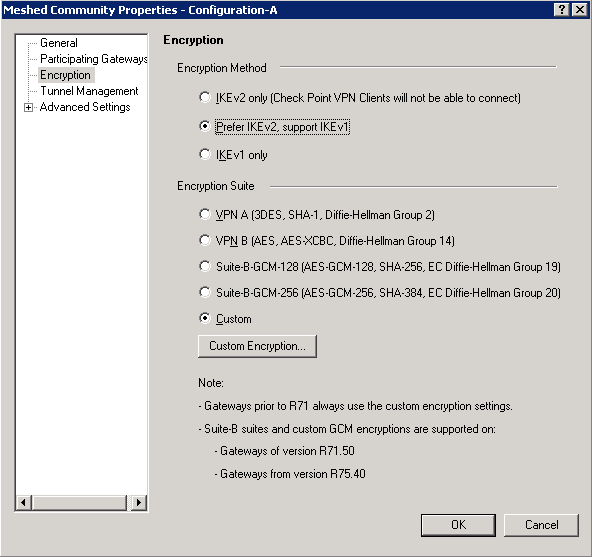
\includegraphics{checkpoint_1.png}

Either chose one of the encryption suites here, or proceed to
``Custom Encryption...'', where you can set encryption and hash for
Phase 1 and 2:

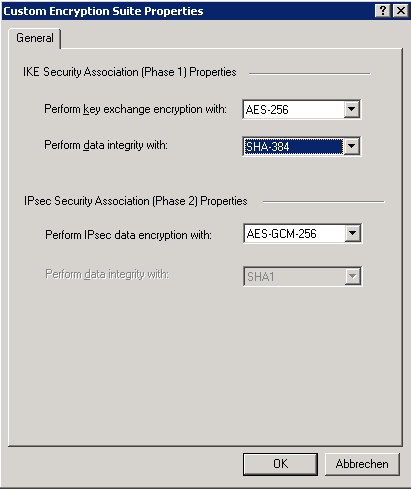
\includegraphics{checkpoint_2.png}

The Diffie-Hellman groups and Perfect Forward Secrecy Settings can be
found under ``Advanced Settings'' / ``Advanced VPN Properties'':

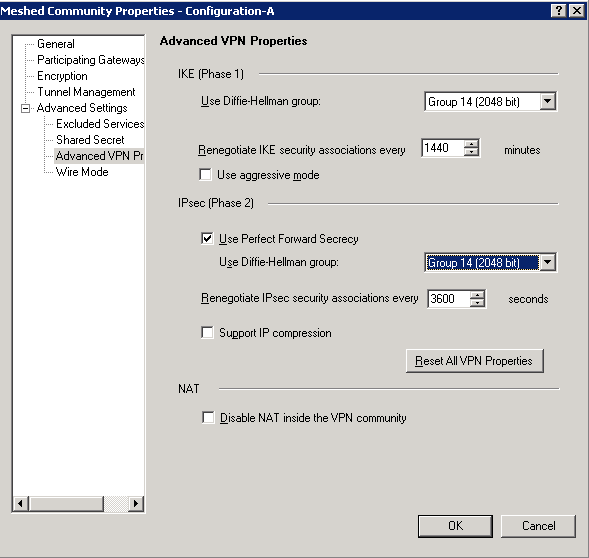
\includegraphics{checkpoint_3.png}

\item[Additional settings:]

For remote Dynamic IP Gateways, the settings are not taken from the
community, but set in the ``Global Properties'' dialog under ``Remote
Access'' / ``VPN Authentication and Encryption''. Via the ``Edit...''
button, you can configure sets of algorithms that all gateways support:

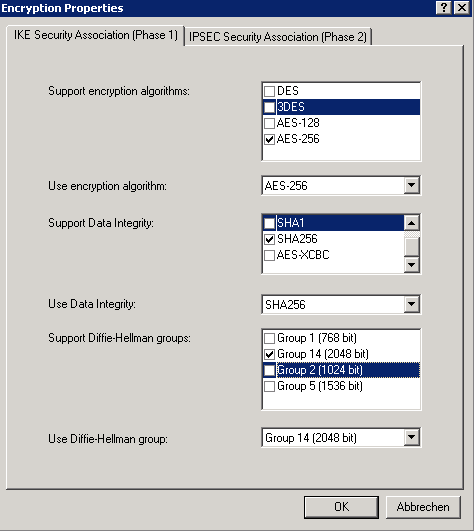
\includegraphics{checkpoint_4.png}

Please note that these settings restrict the available algorithms for
\textbf{all} gateways, and also influence the VPN client connections.

%\item[Justification for special settings (if needed):]

%\item[Limitations:]

\item[References:]\mbox{}

\begin{itemize}

\item Check Point
  \href{https://sc1.checkpoint.com/documents/R77/CP_R77_VPN_AdminGuide/html_frameset.htm}{VPN
    R77 Administration Guide} (may require a
  UserCenter account to access)

\end{itemize}

% \item[How to test:]

\end{description}


\subsubsection{OpenVPN}

\begin{description}

\item[Tested with Version:] OpenVPN 2.3.2 from Debian backports linked against openssl (libssl.so.1.0.0) 

\todo{cm: please write this subsubsection}
\todo{We suppose user uses easy-rsa which is roughly used in all HOWTO\footnote{\url{http://openvpn.net/index.php/open-source/documentation/howto.html}}}


\item[Additional settings:] \mbox{}

\paragraph{Fine tuning at installation level}

When installing an OpenVPN server instance, you are probably using {\it easy-rsa} tools to generate the crypto stuff needed.
From the directory where you will run them, you can enhance you configuration by changing the following variables in \verb|vars|:

\begin{lstlisting}[breaklines]
export KEY_SIZE=2048 
export KEY_EXPIRE=365
export CA_EXPIRE=1826
\end{lstlisting}

This will enhance the security of the key generation by using RSA keys
with a length of 2048 bits, and set a lifetime of one year for the
keys and five years for the CA certificate.

In addition, edit the \verb|pkitool| script and replace all occurences
of \verb|sha1| with \verb|sha256|, to sign the certificates with
SHA256.

\paragraph{Server Configuration}

In the server configuration file, you can select the algorithm that will be used for traffic encryption.
Based on previous recommendation established in that document, select AES with a 256 bits key in CBC mode.

Note that TLS is used only for negotiation bla bla bla...

\todo{cm: explain how openvpn crypto works; make configA/B sections/tables}

\item[Settings:] \mbox{}

% openvpn --show-ciphers
% --show-tls

\todo{cm: changelog 2.3.1: ``Switch to IANA names for TLS ciphers'' --
give both types of strings?}

\begin{lstlisting}[breaklines]
cipher AES-256-CBC   # AES

# TLS Authentication
tls-auth ta.key
tls-cipher EECDH+aRSA+AESGCM:EECDH+aRSA+SHA384:EECDH+aRSA+SHA256:EDH+CAMELLIA256:EECDH:EDH+aRSA:+SSLv3:!aNULL:!eNULL:!LOW:!3DES:!MD5:!EXP:!PSK:!SRP:!DSS:!RC4:!SEED:!AES128:!CAMELLIA128:!ECDSA:AES256-SHA

auth SHA512

reneg-bytes XXX
reneg-pkts XXX
reneg-sec XXX

\end{lstlisting}

% tls-cipher is a list, C&P the string!
% what about: TLS-DHE-RSA-WITH-AES-256-CBC-SHA
% DH params/DH key sizes

\todo{Explain a little bit tls-auth and auth directives + TEST}
\todo{also test with network-damager?}

The following ciphers are avaible and recommended\footnote{You can retrieve the list of supported algorithm on your OpenVPN installation thanks to the command {\it openvpn --show-ciphers}}
\begin{lstlisting}[breaklines]
AES-128-CBC
AES-192-CBC
AES-256-CBC
CAMELLIA-128-CBC
CAMELLIA-192-CBC
CAMELLIA-256-CBC
SEED-CBC
\end{lstlisting}


\paragraph{Client Configuration}

Client and server have to use identical configuration otherwise they can't communicate.
The {\it cipher} directive has then to be identical in both server and client configuration.

\begin{lstlisting}[breaklines]
cipher AES-256-CBC   # AES

remote-cert-tls server # http://openvpn.net/index.php/open-source/documentation/howto.html#mitm

tls-remote server.example.com

\end{lstlisting}

\todo{what about tls-auth keys/ta.key? }. 
\todo{what about auth sha512 ?}

\item[Justification for special settings (if needed):]

\item[References:] \url{http://openvpn.net/index.php/open-source/documentation/security-overview.html}

\item[How to test:]
\todo{write me please}


\end{description}


\subsubsection{PPTP}

PPTP is considered insecure, Microsoft recommends to ``use a more secure VPN
tunnel''\footnote{\url{http://technet.microsoft.com/en-us/security/advisory/2743314}}.

There is a cloud service that cracks the underlying MS-CHAPv2
authentication protocol for the price of USD~200\footnote{\url{https://www.cloudcracker.com/blog/2012/07/29/cracking-ms-chap-v2/}},
and given the resulting MD4 hash, all PPTP traffic for a user can
be decrypted.

\subsubsection{Cisco IPSec}
\todo{write this subsubsection}

\subsubsection{Juniper VPN}
\todo{write this subsubsection. AK: ask Hannes}

\subsubsection{L2TP over IPSec}
\todo{write this subsubsection}

\subsubsection{Racoon}
\todo{write this subsubsection}


\subsection{PGP/ GPG - Pretty Good Privacy}

\todo{re-work this subsection -- this is still only a draft!!}
% hack.
\gdef\currentsectionname{GPG}
\gdef\currentsubsectionname{GnuPG}

The OpenPGP protocol\footnote{\url{https://tools.ietf.org/search/rfc4880}} defines a set of asymmetric- and symmetric encryption algorithms, signature methods and compression protocols. GnuPG\footnote{\url{https://gnupg.org/}}, a FOSS implementation of the OpenPGP standard, is widely used for mail encryption.
 
GnuPG signs a message (SHA-2, RIPEMD or SHA-1), encrypts it symmetrically (AES, CAMELLIA, TWOFISH, BLOWFISH, 3DES, CAST5 or IDEA) and encrpts the symmetric key and the hash with Bob's public key asymmetrically (RSA, ELG, DSA, ECDH, ECDSA or EDDSA).

Research on SHA-1 conducted back in 2005\footnote{\url{https://www.schneier.com/blog/archives/2005/02/sha1\_broken.html}} as well as the first practical successful collision in early 2017\footnote{\url{https://shattered.io/}} has made clear that collision attacks are a real threat to the security of the SHA-1 hash function. Since SHA-1 is defined as a must implementation by the OpenPGP specification, GnuPG is still using it. Currently settings should be adapted to preferably avoid using SHA-1. 

When using GnuPG, there are a couple of things to take care of:
\begin{itemize*}
  \item keylengths (see section \ref{section:keylengths})
  \item randomness (see section \ref{section:RNGs})
  \item preference of symmetric encryption algorithm (see section \ref{section:CipherSuites})
  \item preference of hash function (see section \ref{section:CipherSuites})
\end{itemize*}

Properly dealing with key material, passphrases and the web-of-trust is outside of the scope of this document. The GnuPG website\footnote{\url{http://www.gnupg.org}} has a good tutorial on PGP.

This \href{https://www.debian-administration.org/users/dkg/weblog/48}{Debian How-to}\footnote{\url{https://www.debian-administration.org/users/dkg/weblog/48}} is a great resource on upgrading your old PGP key as well as on safe default settings. This section is built based on the Debian How-to.

\subsubsection{Hashing}
Avoid SHA-1 by prefering better hashing methodes. GnuPG. Edit \$HOME/.gnupg/gpg.conf:

\configfile{gpg.conf}{208-210}{Digest selection in GnuPG}

Before you generate a new OpenPGP key, make sure there is enough entropy available (see subsection \ref{subsec:RNG-linux}).

\subsection{Key Generation}
\gdef\currentsectionname{GPG}
\gdef\currentsubsectionname{GnuPG}
Because of lack of forward secrecy\ac{PFS} in OpenPGP it is preferable to use large asymmetric keys for long term
communication protection. A RSA key of 8192 bits should provide enough confidentiallity for the next 15+ years\footnote{\url{https://www.keylength.com}}.

\configfile{new-key-generation.txt}{}{New key generation with GnuPG version 2.1}

\configfile{params.txt}{}{Paramters for key generation with GnuPG version 2.1}

\subsection{ECC - Ellyptic Curve Cryptography}
Since the realease of GnuPG version 2.1 end-2014\footnote{\url{https://www.gnupg.org/faq/whats-new-in-2.1.html}} ECC is supported. Older versions though are still widely used therefore ECC is not yet applicable in practice. 

%\subsubsection{PGP / GPG Operations}

%% Ciphering - Unciphering operations
%%% TOO COMPLEX. Make a pointer to a good GPG tutorial

%% Signing / checking signatures
%%% TOO COMPLEX. Make a pointer to a good GPG tutorial

%\subsubsection{Trusted Keys}

%%Explain that a key by himself is not trustable.  Chain of trust principle.

%%% TOO COMPLEX. Make a pointer to a good GPG tutorial

%\subsection{Available implementations and mails plugins}

%% Microsoft Windows (Symantec for Outlook? GnuPG + ....)
%%% TOO COMPLEX. Make a pointer to a good GPG tutorial

%% Linux (GnuPG + Enigmail for Thunderbird)

%%% TOO COMPLEX. Make a pointer to a good GPG tutorial
%% Mac OS X (GnuPG + GPGMail)
%%% TOO COMPLEX. Make a pointer to a good GPG tutorial




\subsection{seclayer-tcp}
\todo{Ramin: please write this section or ask Posch}
For the austrian citizen card....

\begin{verbatim}
seclayer-tcp    3495/udp    # securitylayer over tcp
seclayer-tcp    3495/tcp    # securitylayer over tcp
\end{verbatim}


\subsection{IPMI, ILO and other lights out management solutions}


We \textbf{strongly} recommend that any remote management system for servers such as ILO, IPMI and similar never be connected to a public IP address.
Consider creating a management VLAN and access that only via a VPN.


\subsection{SIP}
\todo{AK: ask Klaus. Write this section, Klaus??? }

\subsection{Instant Messaging Systems}
\subsubsection{XMPP / Jabber}
\todo{ts: Describe ejabberd configuration. Reference to Peter`s manifesto https://github.com/stpeter/manifesto}
\subsubsection{IRC}

%%\subsection{Database Systems}
% This list is based on : http://en.wikipedia.org/wiki/Relational_database_management_system#Market_share

\subsubsection{Oracle}
\todo{write this}

\subsubsection{SQL Server}
\todo{write this}




\subsubsection{MySQL}

\begin{description}
\item[Tested with Version:] Debian 7.0 and MySQL 5.5

\item[Settings:] \mbox{}

\paragraph*{my.cnf}\mbox{}\\

\begin{lstlisting}[breaklines]
[mysqld]
ssl
ssl-ca=/etc/mysql/ssl/ca-cert.pem
ssl-cert=/etc/mysql/ssl/server-cert.pem
ssl-key=/etc/mysql/ssl/server-key.pem
ssl-cipher=EECDH+aRSA+AESGCM:EECDH+aRSA+SHA384:EECDH+aRSA+SHA256:EDH+CAMELLIA256:EECDH:EDH+aRSA:+SSLv3:!aNULL:!eNULL:!LOW:!3DES:!MD5:!EXP:!PSK:!SRP:!DSS:!RC4:!SEED:!AES128:!CAMELLIA128:!ECDSA:AES256-SHA
\end{lstlisting}

\item[Additional settings:]


\item[Justification for special settings (if needed):]

% in case you have the need for further justifications why you chose this and that setting or if the settings do not fit into the standard Variant A or Variant B schema, please document this here

\item[References:]
+{\small \url{https://dev.mysql.com/doc/refman/5.5/en/ssl-connections.html}}


% add any further references or best practice documents here

\item[How to test:]

After restarting the server run the following query to see if the ssl settings are correct:
\begin{lstlisting}[breaklines]
show variables like '%ssl%';
\end{lstlisting}


\end{description}






\subsubsection{DB2}
\todo{write this}





\subsubsection{Postgresql}

\begin{description}
\item[Tested with Version:] Debian 7.0 and PostgreSQL 9.1

\item[References:]

It's recommended to read 

{\small \url{http://www.postgresql.org/docs/current/static/runtime-config-connection.html#RUNTIME-CONFIG-CONNECTION-SECURITY}}
{\small \url{http://www.postgresql.org/docs/current/static/ssl-tcp.html}}
{\small \url{http://www.postgresql.org/docs/current/static/auth-pg-hba-conf.html}}

\item[Settings:] \mbox{}


To start in SSL mode the server.crt and server.key must exist in the server's data directory \$PGDATA. 

Starting with version 9.2, you have the possibility to set the path.

\begin{lstlisting}[breaklines]
ssl_key_file = '/your/path/server.key'
ssl_cert_file = '/your/path/server.crt'
ssl_ca_file = '/your/path/root.crt'
\end{lstlisting}

\paragraph*{postgresql.conf}\mbox{}\\

\begin{lstlisting}[breaklines]
#>=8.3
ssl = on 
ssl_ciphers = 'EECDH+aRSA+AESGCM:EECDH+aRSA+SHA384:EECDH+aRSA+SHA256:EDH+CAMELLIA256:EECDH:EDH+aRSA:+SSLv3:!aNULL:!eNULL:!LOW:!3DES:!MD5:!EXP:!PSK:!SRP:!DSS:!RC4:!SEED:!AES128:!CAMELLIA128:!ECDSA:AES256-SHA'
\end{lstlisting}



\item[How to test:]
To test your ssl settings, run psql with the sslmode parameter:
\begin{lstlisting}[breaklines]
psql "sslmode=require host=postgres-server dbname=database" your-username
\end{lstlisting}

\end{description}




\subsubsection{Informix}
\todo{write this}


%hack.
\gdef\currentsectionname{Proxies}
%%\subsection{Intercepting proxy solutions and reverse proxies}

Within enterprise networks and corporations with increased levels of paranoia or at least some defined security requirements it is common \textbf{not} to allow direct connections to the public internet.

For this reason proxy solutions are deployed on corporate networks to intercept and scan the traffic for potential threats within sessions.

For encrypted traffic there are four options:

\begin{itemize*}
  \item Block the connection because it cannot be scanned for threats.
  \item Bypass the threat-mitigation and pass the encrypted session to the client, which results in a situation where malicious content is transferred directly to the client without visibility to the security system.
  \item Intercept (i.e. terminate) the session at the proxy, scan there and re-encrypt the session towards the client (effectively MITM).
  \item Deploy special Certificate Authorities to enable Deep Packet Inspection on the wire.
\end{itemize*}

While the latest solution might be the most "up to date", it arises a new front in the context of this paper, because the most secure part of a client's connection could only be within the corporate network, if the proxy-server handles the connection to the destination server in an insecure manner.

Conclusion: Don't forget to check your proxy solutions SSL-capabilities. Also do so for your reverse proxies!

%% ---------------------------------------------------------------------- 
% who was the author of this section?
% can we have this either tested or removed?
%\subsection{Squid}
%As of squid-3.2.7 (01 Feb 2013) there is support for the OpenSSL NO\_Compression option within squid config (CRIME attack) and if you combine that in the config file, with an enforcement of the server cipher preferences (BEAST Attack) you are safe.
%
%
%\todo{UNTESTED!}
%\configfile{squid.conf}{1363-1363,1379-1379}{Cipher selection and SSL options in Squid}
%%% http://forum.pfsense.org/index.php?topic=63262.0
%%\todo{UNTESTED!}
%% see squid.conf, repeating the options here does not help.
%\todo{Patch here? Definitely working for 3.2.6!}
%For squid Versions before 3.2.7 use this patch against a vanilla source-tree:
%\begin{lstlisting}
%--- support.cc.ini      2013-01-09 02:41:51.000000000 +0100
%+++ support.cc  2013-01-21 16:13:32.549383848 +0100
%@@ -400,6 +400,11 @@
%         "NO_TLSv1_2", SSL_OP_NO_TLSv1_2
%     },
% #endif
%+#ifdef SSL_OP_NO_COMPRESSION
%+    {
%+        "NO_Compression", SSL_OP_NO_COMPRESSION
%+    },
%+#endif
%     {
%         "", 0
%     },
%\end{lstlisting}
%
%
%% ---------------------------------------------------------------------- 
\subsection{Bluecoat}
%% https://kb.bluecoat.com/index?page=content&id=KB5549
\subsubsection{Tested with Versions}
\begin{itemize*}
  \item SGOS 6.5.x
\end{itemize*}

BlueCoat Proxy SG Appliances can be used as forward and reverse proxies. The reverse proxy feature is rather under-developed, and while it is possible and supported, there only seems to be limited use of this feature "in the wild" - nonetheless there are a few cipher suites to choose from, when enabling SSL features.

\paragraph*{Only allow TLS 1.0,1.1 and 1.2 protocols:}
~
\begin{lstlisting}
$conf t
$(config)ssl
$(config ssl)edit ssl-device-profile default
$(config device-profile default)protocol tlsv1 tlsv1.1 tlsv1.2
  ok
\end{lstlisting}

\paragraph*{Select your accepted cipher-suites:}
~
\begin{lstlisting}
$conf t
Enter configuration commands, one per line.  End with CTRL-Z.
$(config)proxy-services
$(config proxy-services)edit ReverseProxyHighCipher
$(config ReverseProxyHighCipher)attribute cipher-suite
Cipher#  Use        Description        Strength
-------  ---  -----------------------  --------
      1  yes            AES128-SHA256      High
      2  yes            AES256-SHA256      High
      3  yes               AES128-SHA    Medium
      4  yes               AES256-SHA      High
      5  yes       DHE-RSA-AES128-SHA      High
      6  yes       DHE-RSA-AES256-SHA      High
               [...]
     13  yes          EXP-RC2-CBC-MD5    Export

Select cipher numbers to use, separated by commas: 2,5,6
  ok
\end{lstlisting}

The same protocols are available for forward proxy settings and should be adjusted accordingly:
In your local policy file add the following section:
\begin{lstlisting}
<ssl>
    DENY server.connection.negotiated_ssl_version=(SSLV2, SSLV3)
\end{lstlisting}

Disabling protocols and ciphers in a forward proxy environment could lead to unexpected results on certain (misconfigured?) webservers (i.e. ones accepting only SSLv2/3 protocol connections)


%% ---------------------------------------------------------------------- 
\subsection{HAProxy}
% See http://www.haproxy.org/

HAProxy can be used as loadbalancer and proxy for TCP and HTTP-based applications. Since version 1.5 it supports SSL and IPv6.

\subsubsection{Tested with Versions}
\begin{itemize*}
  \item HAProxy 1.5.11 with OpenSSL 1.0.1e on Debian Wheezy
\end{itemize*}

\subsubsection{Settings}
\configfile{haproxy.cfg}{1-4}{global configuration}
\configfile{haproxy.cfg}{21-25}{frontend configuration}
\configfile{haproxy.cfg}{27-33}{backend configuration}


%% ---------------------------------------------------------------------- 
\subsection{Pound}
% See http://www.apsis.ch/pound
% See https://help.ubuntu.com/community/Pound

\subsubsection{Tested with Versions}
\begin{itemize*}
  \item Pound 2.6
\end{itemize*}

\subsubsection{Settings}
\configfile{pound.cfg}{31}{HTTPS Listener in Pound}


%% ---------------------------------------------------------------------- 
\subsection{stunnel}
% See https://www.stunnel.org/

\subsubsection{Tested with Versions}
\begin{itemize*}
  \item stunnel 4.53-1.1ubuntu1 on Ubuntu 14.04 Trusty with OpenSSL 1.0.1f, without disabling Secure Client-Initiated Renegotiation
  \item stunnel 5.02-1 on Ubuntu 14.04 Trusty with OpenSSL 1.0.1f
  \item stunnel 4.53-1.1 on Debian Wheezy with OpenSSL 1.0.1e, without disabling Secure Client-Initiated Renegotiation
\end{itemize*}

\subsubsection{Settings}
\configfile{stunnel.conf}{48-55}{HTTPS Listener in Pound}

\subsubsection{Additional information}
Secure Client-Initiated Renegotiation can only be disabled for stunnel versions >= 4.54, when the renegotiation parameter has been added (See changelog).

\subsubsection{References} 
\begin{itemize*}
  \item stunnel documentation: \url{https://www.stunnel.org/static/stunnel.html}
  \item stunnel changelog: \url{https://www.stunnel.org/sdf_ChangeLog.html}
\end{itemize*}


\subsubsection{How to test} 
See appendix \ref{cha:tools}

 



%%% Local Variables: 
%%% mode: latex
%%% TeX-master: "applied-crypto-hardening"
%%% End: 
